\documentclass{beamer}
\usefonttheme[onlymath]{serif}
\usepackage[T1]{fontenc}
\usepackage[utf8]{inputenc}
\usepackage[english, icelandic]{babel}
\usepackage{amsmath}
\usepackage{amssymb}
\usepackage{amsthm}
\usepackage{gensymb}
\usepackage{parskip}
\usepackage{mathtools}
\usepackage{xfrac}
\usepackage{graphicx}
\usepackage{xcolor}
\usepackage{tikz}
\usetikzlibrary{calc}
\usetikzlibrary{positioning}
\usepackage{verbatim}
\usepackage{multicol}
\usepackage{minted}
\parskip 0pt

\DeclareMathOperator{\lcm}{lcm}
\DeclareMathOperator{\diam}{diam}
\DeclareMathOperator{\dist}{dist}
\DeclareMathOperator{\ord}{ord}
\DeclareMathOperator{\Aut}{Aut}
\DeclareMathOperator{\Inn}{Inn}
\DeclareMathOperator{\Ker}{Ker}
\DeclareMathOperator{\trace}{trace}
\DeclareMathOperator{\fix}{fix}
\DeclareMathOperator{\Log}{Log}
\newcommand\floor[1]{\left\lfloor#1\right\rfloor}
\newcommand\ceil[1]{\left\lceil#1\right\rceil}
\newcommand\abs[1]{\left|#1\right|}
\newcommand\p[1]{\left(#1\right)}
\newcommand\sqp[1]{\left[#1\right]}
\newcommand\cp[1]{\left\{#1\right\}}
\newcommand\norm[1]{\left\lVert#1\right\rVert}
\renewcommand\qedsymbol{$\blacksquare$}
\renewcommand\Im{\operatorname{Im}}
\renewcommand\Re{\operatorname{Re}}

\usetheme{Madrid}
\definecolor{dark yellow}{rgb} {0.6,0.6,0.0}
\definecolor{dark green}{rgb} {0.0,0.6,0.0}

\title{Netafræði II}
\subtitle{Stefnd og vigtuð net}
\author{Atli Fannar Franklín}
\date{\today}

\graphicspath{{myndir/}}

\AtBeginSection[] {
  \begin{frame}
    \frametitle{Efnisyfirlit}
    \tableofcontents[currentsection]
  \end{frame}
}


\begin{document}

\frame{\titlepage}

\section[Grunnatriði]{Grunnatriði}

\begin{frame}
\frametitle{Hvað er stefnt eða vigtað net?}

\begin{itemize}

\item<1-> Stefnt net er net þar sem leggirnir hafa stefnu, þ.e.a.s. þeir liggja frá einum hnút til annars en ekki til baka. Þetta getur táknað einstefnur eða aðra ferðamáta sem virka bara í eina átt, hlutir að flæða í eina átt, hver sigrar hvern og margt fleira.

\item<2-> Vigtað net er net þar sem leggirnir hafa þyngd (eða lengd) sem er einhver rauntala. Þetta getur táknað lengd vegarins sem svarar til leggjarins, kostnað við að smíða legginn, um hversu mikið annar leikmaður vann hinn og margt fleira.

\item<3-> Net geta verið óstefnd og óvigtuð, óstefnd og vigtuð, stefnd og óvigtuð eða stefnd og vigtuð. Í öllum þessum tilvikum geta þau verið einföld eða ekki.

\end{itemize}

\end{frame}

\begin{frame}
\frametitle{Dæmi um stefnt vigtað net}

\begin{center}
\hspace*{-1.5cm}
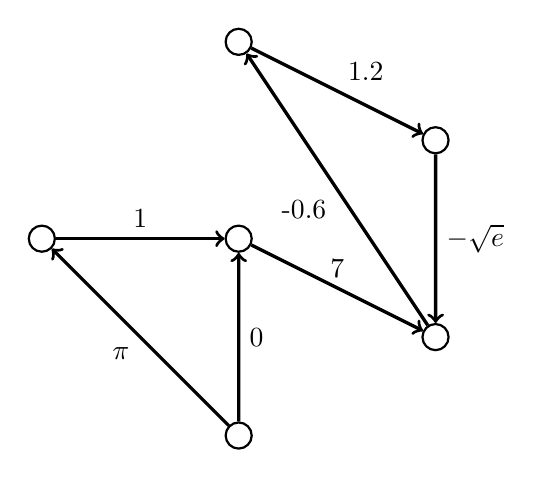
\begin{tikzpicture}[scale=1.25]

\node[draw, circle, thick] (1) at (0,0) {};
\node[draw, circle, thick] (2) at (2,0) {};
\node[draw, circle, thick] (3) at (2,2) {};
\node[draw, circle, thick] (4) at (2,-2) {};
\node[draw, circle, thick] (5) at (4,1) {};
\node[draw, circle, thick] (6) at (4,-1) {};

\path[draw, ->, very thick] (1) -- node[midway, above] {1} (2);
\path[draw, ->, very thick] (2) -- node[midway, above] {7} (6);
\path[draw, ->, very thick] (3) -- node[midway, above right] {1.2} (5);
\path[draw, ->, very thick] (4) -- node[midway, below left] {$\pi$} (1);
\path[draw, ->, very thick] (6) -- node[midway, below left] {-0.6} (3);
\path[draw, ->, very thick] (4) -- node[midway, right] {0} (2);
\path[draw, ->, very thick] (5) -- node[midway, right] {$-\sqrt{e}$} (6);

\end{tikzpicture}
\end{center}

\end{frame}

\begin{frame}
\frametitle{Framsetning}

\begin{itemize}

\item<1-> Nágrannaframseting er geymd með sama hætti í stefndu neti nema við geymum bara að $a$ sé nágranni $b$ ef örin liggur í þá átt en ekki öfugt. Ef netið er vigtað er hægt að geyma tvenndir $(n, w)$ í listanum þar sem $n$ er nágrannin og $w$ er vigt örvarinnar þangað. Notum þetta áfram mest.

\item<2-> Í fylkjaframsetningu getum við bara geymt einföld vigtuð net eða óvigtuð net. Ef þau eru vigtuð látum við töluna í $A[i][j]$ vera vigt leggjarins í stað fjölda leggja. Við getum þá ekki heldur haft vigtir sem eru 0 nema við látum $\infty$ tákna enga leggi. Ef netið er stefnt setjum við bara $A[i][j]$ sem legginn frá $i$ til $j$ en $A[j][i]$ sem legginn frá $j$ til $i$.

\item<3-> Í listaframsetningu breytist lítið. Ef netið er stefnt táknar þá $(a, b)$ legg frá $a$ til $b$ en ekki öfugt. Ef netið er vigtað notum við þrenndir $(a, b, w)$ í stað tvennda og geymum þá vigtina $w$ aftast.

\end{itemize}

\end{frame}

\section[Reiknirit á stefndum óvigtuðum netum]{Reiknirit á stefndum óvigtuðum netum}

\begin{frame}
\frametitle{Hvað getum við gert nýtt á stefndu neti?}

\begin{itemize}

\item<1-> Við getum skoðað samhengisþætti í nýju ljósi. Við getum talað um stranglega samanhangandi þætti (SCC) sem eru hlutar stefnds nets þar sem við komumst milli sérhverra tveggja hnúta þess.

\item<2-> Með þessu getum við líka látið alla slíka samhengisþætti skreppa saman í einn hnút og köllum við það herpingu nets. Við það að gera þetta fæst svokallað órásað stefnt net (DAG), sem þýðir einfaldlega að ekki sé hægt að fara í hring í netinu ef ferðast er meðfram örvunum.

\item<3-> Skulum sjá dæmi um stranglega samanhangandi þætti, herpingu og órásað stefnt net.

\end{itemize}

\end{frame}

\begin{frame}
\frametitle{Stranglega samanhangandi þættir}

\begin{center}
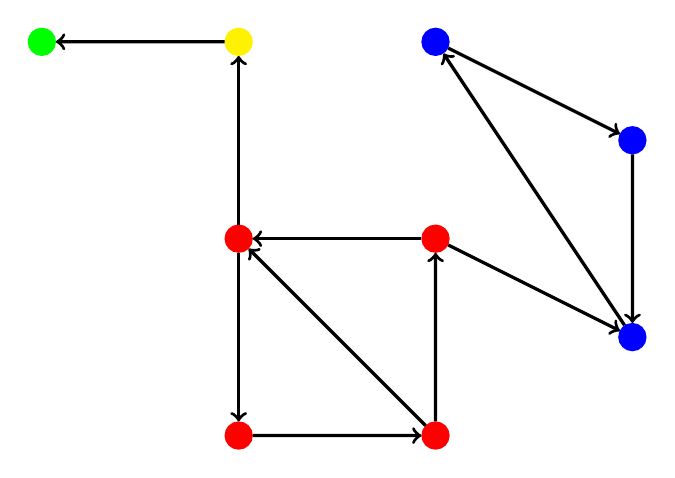
\begin{tikzpicture}[scale=1.25]

\node[draw, circle, thick, red, fill] (1) at (0,0) {};
\node[draw, circle, thick, red, fill] (2) at (2,0) {};
\node[draw, circle, thick, blue, fill] (3) at (2,2) {};
\node[draw, circle, thick, red, fill] (4) at (2,-2) {};
\node[draw, circle, thick, blue, fill] (5) at (4,1) {};
\node[draw, circle, thick, blue, fill] (6) at (4,-1) {};
\node[draw, circle, thick, red, fill] (7) at (0,-2) {};
\node[draw, circle, thick, yellow, fill] (8) at (0,2) {};
\node[draw, circle, thick, green, fill] (9) at (-2,2) {};

\path[draw, ->, very thick] (2) -- (1);
\path[draw, ->, very thick] (2) -- (6);
\path[draw, ->, very thick] (3) -- (5);
\path[draw, ->, very thick] (4) -- (1);
\path[draw, ->, very thick] (6) -- (3);
\path[draw, ->, very thick] (4) -- (2);
\path[draw, ->, very thick] (5) -- (6);
\path[draw, ->, very thick] (1) -- (8);
\path[draw, ->, very thick] (8) -- (9);
\path[draw, ->, very thick] (1) -- (7);
\path[draw, ->, very thick] (7) -- (4);

\end{tikzpicture}
\end{center}

\end{frame}

\begin{frame}
\frametitle{Herping}

\begin{center}
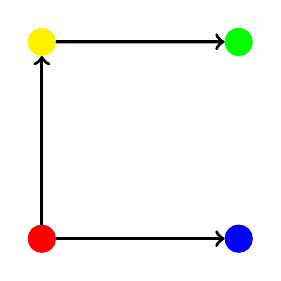
\begin{tikzpicture}[scale=1.25]

\node[draw, circle, thick, red, fill] (1) at (0,0) {};
\node[draw, circle, thick, blue, fill] (2) at (2,0) {};
\node[draw, circle, thick, yellow, fill] (3) at (0,2) {};
\node[draw, circle, thick, green, fill] (4) at (2,2) {};

\path[draw, ->, very thick] (1) -- (2);
\path[draw, ->, very thick] (1) -- (3);
\path[draw, ->, very thick] (3) -- (4);

\end{tikzpicture}
\end{center}

\end{frame}

\begin{frame}
\frametitle{Ákvörðun stranglegra samanhangandi þátta}

\begin{itemize}

\item<1-> Oft er nytsamlegt að ákvarða stranglega samanhangandi þætti nets. En hvernig má gera það?

\item<2-> Við getum breytt reikniritinu úr síðasta fyrirlestri sem finnur brýr og tengihnúta til þess að gera þetta.

\item<3-> Þetta vinnur útfrá því að ef leggur er brú er engin leið að komast til baka skv. skilgr. brúar, svo endahnútar brúarinnar verða að vera í ólíkum stranglega samanhangandi þáttum.

\item<4-> Þetta til viðbótar við það að skoða hvenær við komumst til baka í fyrri hnút gefur okkur reiknirit Tarjans til að finna stranglega samanhangandi þætti.

\item<5-> Útfærslan í bókinni skilar lista af listum þar sem hver listi er einn stranglega samanhangandi þáttur. Í minni útfærslu skila ég union-find tilviki í staðinn. Útfærslan dregur einkenni sín af útfærslu Bjarka Ágústs Guðmundssonar.

\end{itemize}

\end{frame}

\begin{frame}[fragile]
\frametitle{Reiknirit Tarjans}

\begin{columns}
\begin{column}{0.5\textwidth}
\begin{tiny}
\begin{minted}{cpp}
#include<bits/stdc++.h>
using namespace std;
typedef vector<int> vi;
typedef vector<vi> vvi;

struct union_find {
  vi p; union_find(int n) : p(n, -1) { }
  int find(int x) { 
      return p[x] < 0 ? x : p[x] = find(p[x]); }
  bool united(int x, int y) { 
      return find(x) == find(y); }
  void unite(int x, int y) {
    int xp = find(x), yp = find(y);
    if (xp == yp) return;
    if (p[xp] > p[yp]) swap(xp,yp);
    p[xp] += p[yp], p[yp] = xp;
    return; }
int size(int x) { return -p[find(x)]; } };

vi ord;
vector<bool> done;

void dfs(vvi& g, int v) {
    done[v] = true;
    for(int x : g[v]) if(!done[x]) dfs(g, x);
    ord.push_back(v);
}
\end{minted}
\end{tiny}
\end{column}

\begin{column}{0.5\textwidth}
\begin{tiny}
\begin{minted}{cpp}
pair<union_find, vi> tarjan(vvi& g) {
    ord.clear();
    union_find uf(g.size());
    vi dag; vvi gr(g.size());
    for(int i = 0; i < g.size(); ++i) {
        for(int x : g[i]) {
            gr[x].push_back(i);
        }
    }
    done.resize(g.size());
    for(int i = 0; i < g.size(); ++i) 
        done[i] = false;
    for(int i = 0; i < g.size(); ++i) 
        if(!done[i]) dfs(gr, i);
    for(int i = 0; i < g.size(); ++i) 
        done[i] = false;
    stack<int> s;
    for(int i = g.size() - 1; i >= 0; --i) {
        if(done[ord[i]]) continue;
        s.push(ord[i]); dag.push_back(ord[i]);
        while(!s.empty()) {
            int t = s.top();
            done[t] = true;
            s.pop();
            uf.unite(t, ord[i]);
            for(int x : g[t]) {
                if(!done[x]) s.push(x);
            }
        }
    }
    reverse(dag.begin(), dag.end());
    return make_pair(uf, dag);
}
\end{minted}
\end{tiny}
\end{column}
\end{columns}

\end{frame}

\begin{frame}[fragile]
\frametitle{Prófun á Tarjan}

\begin{columns}
\begin{column}{0.5\textwidth}
\begin{small}
\begin{minted}{cpp}
int main() {
    int n, m, a, b;
    cin >> n >> m;
    vvi g(n, vi());
    for(int i = 0; i < m; ++i) {
        cin >> a >> b;
        g[a].push_back(b);
    }
    auto t = tarjan(g);
    for(int x : t.first.p) {
        cout << x << ' ';
    }
    cout << endl;
    for(int x : t.second) {
        cout << x << ' ';
    }
    cout << endl;
}
\end{minted}
\end{small}
\end{column}

\begin{column}{0.5\textwidth}
\begin{minted}{cpp}
// Inntak
9 11
1 0
3 1
2 3
2 1
0 2
1 7
7 8
3 4
4 5
5 6
6 4
// Úttak
2 2 -4 2 5 -3 5 -1 -1 
0 4 7 8 
\end{minted}
\end{column}
\end{columns}

\end{frame}

\begin{frame}
\frametitle{DAG?}

\begin{itemize}

\item<1-> Tarjan keyrir almennt í $\mathcal{O}(E + V)$, í minni útfærslu er það í raun $\mathcal{O}(E + V\alpha(V))$ út af union-find en það er í öllum raunhæfum tilfellum varla neinn munur þar á.

\item<2-> En hvað er þetta \texttt{dag} sem ég skila líka? Eins og kom fram áðan er DAG órásað stefnt net. Það merkilega við slík net er að raða má hnútunum í röð (ekki endilega ótvírætt ákvarðaða) þ.a. ef til er leggur frá $a$ til $b$ verður $b$ að vera á eftir $a$ í röðinni.

\item<3-> Þetta kallast grannröðun (topological sort). Reikniritið hér á undan gefur okkur sem sagt grannröðun á herpingu netsins frítt með!

\item<4-> En hvað ef við viljum grannröðun á neti sem þegar er órásað? Það myndi virka að keyra reikniritið að ofan því þá yrðu allir hnútar sinn eiginn stranglega samanhangandi þáttur. Það má gera það með smærra forriti sem gerir í raun það sama og að Tarjan, bara með minna bókhaldi. En einnig er hægt að nota reiknirit Kahn's (sjá bók). En þar sem öll þessi reiknirit hafa sömu tímaflækju ($\mathcal{O}(V + E)$), þá látum við þetta duga.

\end{itemize}

\end{frame}

\section[Reiknirit á vigtuðum óstefndum netum]{Reiknirit á vigtuðum óstefndum netum}

\begin{frame}
\frametitle{Spannandi tré}

\begin{itemize}

\item<1-> Fyrsta sem manni dytti í hug væri líklegast að skoða ódýrustu leiðina milli staða. En í ljós kemur að það sé lítill munur á að skoða þetta á stefndu og óstefndu neti ef það er vigtað, svo skoðum það á eftir.

\item<2-> Það sem við getum gert núna er að skoða spurninguna 'Hver er ódýrasta leiðin til að tengja alla hnúta netsins saman?'

\item<3-> Þá veljum við eitthvert hlutmengi leggja sem mynda tré. Af hverju tré? Nú, ef við værum með rás mætti sleppa einhverjum legg í rásinni, sem væri ódýrara.

\item<4-> Svona fyrirbæri köllum við spannandi tré í netinu, og er þá spurningin hvernig við getum ákvarðað lágmarksþyngd á spannandi tré nets.

\end{itemize}

\end{frame}

\begin{frame}
\frametitle{Reiknirit Kruskals}

\begin{itemize}

\item<1-> Þó svo það sé kannski ekki augljóst í fyrstu kemur í ljós að til sé mjög einfalt gráðugt reiknirit til að gera þetta. Er einhver með gisk?

\item<2-> Við bætum alltaf við ódýrasta leggnum sem myndar ekki rás! 

\item<3-> Æfing: sanna að þetta virki.

\item<4-> Við getum þá haldið utan um hvaða leggir hafa veg á milli sín með því að nota union-find. Þá röðum við bara öllum leggjunum í vaxandi þyngdarröð og bætum við þar til allt er orðið tengt og skilum þyngdinni (eða trénu eftir tilvikum). Athugum að net þarf að vera tengt til að slíkt tré sé til. Annars þarf að gera þetta í hverjum samhengisþætti fyrir sig.

\item<5-> Þetta keyrir í $\mathcal{O}(E\log(E))$ ($\alpha$ hverfur því það er minna en $\log$).

\end{itemize}

\end{frame}

\begin{frame}[fragile]
\frametitle{Kruskal útfærsla sem skilar þyngd}

\begin{tiny}
\begin{minted}{cpp}
#include<bits/stdc++.h>
using namespace std;
typedef pair<int,int> ii;
typedef vector<int> vi;
typedef pair<double,ii> dii;
typedef pair<double,int> di;
typedef vector<di> vdi;
typedef vector<vdi> vvdi;
// sama unionfind og síðast

double kruskal(vvdi& g) {
    priority_queue<dii> s; union_find uf(g.size());
    double res = 0;
    for(int i = 0; i < g.size(); ++i)
        for(auto x : g[i]) s.push(dii(-x.first, ii(x.second, i)));
    while(uf.size(0) < g.size()) {
        auto x = s.top(); s.pop();
        if(uf.united(x.second.first, x.second.second)) continue;
        res -= x.first; uf.unite(x.second.first, x.second.second);
    }
    return res; }

int main() {
    int n, m, a, b;
    double w;
    cin >> n >> m;
    vvdi g(n, vdi());
    for(int i = 0; i < m; ++i) {
        cin >> a >> b >> w;
        g[a].push_back(di(w, b));
        g[b].push_back(di(w, a));
    }
    cout << kruskal(g) << endl; }
\end{minted}
\end{tiny}

\end{frame}

\begin{frame}
\frametitle{Hríslur}

\begin{itemize}

\item<1-> Svipað má gera yfir stefnd net.

\item<2-> Þá skoðar maður svokallaðar spannandi hríslur.

\item<3-> Það að skoða spannandi hríslur er töluvert flóknara og kemur mun sjaldnar fyrir í keppnisforritun, svo við sleppum því.

\item<4-> Gott að læra það einhvern tímann samt, eins og við komumst að síðastliðinn nóvember.

\end{itemize}

\end{frame}

\section[Reiknirit á vigtuðum stefndum netum]{Reiknirit á vigtuðum stefndum netum}

\begin{frame}
\frametitle{Leitarreiknirit}

\begin{itemize}

\item<1-> Það sem við munum skoða í restinni á þessum fyrirlestri eru ýmsar leiðir til að finna bestu leið frá $a$ til $b$ í stefndu og vigtuðu neti.

\item<2-> Bendum fyrst á eitt stórt vandamál. Ef til er rás með neikvæða þyngd í netinu er hægt að fara eftir henni aftur og aftur til að fá eins lítinn kostnað og maður vill. Því munum við nú fyrst gera ráð fyrir að við höfum net með ekki neikvæðum vigtum.

\item<3-> Hvernig getum við þá fundið stystu leið frá $a$ til $b$?

\item<4-> Með einu frægasta reikniriti tölvunarfræðinnar, reikniriti Dijkstra!

\end{itemize}

\end{frame}

\begin{frame}
\frametitle{Dijkstra}

\begin{itemize}

\item<1-> Dijkstra finnur stystu leið í alla hnúta frá einum hnút $v$. Það byrjar á því að segja að þessi fjarlægð sé $\infty$ fyrir alla hnúta og að hnúturinn sem við komum úr sé enginn. 

\item<2-> Við geymum svo hnútana sem við eigum eftir að skoða í forgangsbiðröð þar sem forgangurinn er stutt í þá.

\item<3-> Svo meðan biðröðin er ekki tóm tökum við efsta og bætum við nágrönnum þess sem við erum ekki búin að skoða en uppfærum líka fjarlægðina á nágrönnunum ef við erum búin að finna styttri leið. Við uppfærum þá um leið úr hvaða hnút við vorum að koma.

\end{itemize}

\end{frame}

\begin{frame}
\frametitle{Dijkstra in action}

\begin{columns}
\begin{column}{0.65\textwidth}
\begin{tikzpicture}
\only<1>{\node[draw, circle, thick] (1) at (0,3) {1};}
\only<2-5>{\node[draw, circle, thick, dark yellow] (1) at (0,3) {1};}
\only<6->{\node[draw, circle, thick, red] (1) at (0,3) {1};}

\only<1-2>{\node[draw, circle, thick] (2) at (0,1) {2};}
\only<3-5>{\node[draw, circle, thick, dark green] (2) at (0,1) {2};}
\only<6-7>{\node[draw, circle, thick, dark yellow] (2) at (0,1) {2};}
\only<8->{\node[draw, circle, thick, red] (2) at (0,1) {2};}

\only<1-3>{\node[draw, circle, thick] (3) at (2,4) {3};}
\only<4-10>{\node[draw, circle, thick, dark green] (3) at (2,4) {3};}
\only<11-12>{\node[draw, circle, thick, dark yellow] (3) at (2,4) {3};}
\only<13->{\node[draw, circle, thick, red] (3) at (2,4) {3};}

\only<1-4>{\node[draw, circle, thick] (4) at (2,2) {4};}
\only<5-7>{\node[draw, circle, thick, dark green] (4) at (2,2) {4};}
\only<8-10>{\node[draw, circle, thick, dark yellow] (4) at (2,2) {4};}
\only<11->{\node[draw, circle, thick, red] (4) at (2,2) {4};}

\only<1-6>{\node[draw, circle, thick] (5) at (2,0) {5};}
\only<7-12>{\node[draw, circle, thick, dark green] (5) at (2,0) {5};}
\only<13>{\node[draw, circle, thick, dark yellow] (5) at (2,0) {5};}
\only<14->{\node[draw, circle, thick, red] (5) at (2,0) {5};}

\only<1-11>{\node[draw, circle, thick] (6) at (4,2) {6};}
\only<12-13>{\node[draw, circle, thick, dark green] (6) at (4,2) {6};}
\only<14>{\node[draw, circle, thick, dark yellow] (6) at (4,2) {6};}
\only<15>{\node[draw, circle, thick, red] (6) at (4,2) {6};}

\path[draw, ->, very thick] (1) -- node[midway, left] {\footnotesize $6$} (2);
\path[draw, ->, very thick] (1) -- node[midway, above left] {\footnotesize $13$} (3);
\path[draw, ->, very thick] (1) -- node[midway, above right] {\footnotesize $9$}  (4);
\path[draw, ->, very thick] (2) -- node[midway, above left] {\footnotesize $10$} (4);
\path[draw, ->, very thick] (2) -- node[midway, above right] {\footnotesize $15$} (5);
\path[draw, ->, very thick] (3) -- node[midway, above right] {\footnotesize $9$} (6);
\path[draw, ->, very thick] (4) -- node[midway, right] {\footnotesize $2$} (3);
\path[draw, ->, very thick] (4) -- node[midway, right] {\footnotesize $10$} (5);
\path[draw, ->, very thick] (5) -- node[midway, below right] {\footnotesize $4$} (6);

\node[left=0.05cm of 1, blue] {\hspace*{0.25cm}$0$};
\only<1-2>{\node[left=0.05cm of 2, blue] {$\infty$};}
\only<3->{\node[left=0.05cm of 2, blue] {$6$};}
\only<1-3>{\node[right=0.05cm of 3, blue] {$\infty$};}
\only<4-8>{\node[right=0.05cm of 3, blue] {$13$};}
\only<9->{\node[right=0.05cm of 3, blue] {$11$};}
\only<1-4>{\node[right=0.05cm of 4, blue] {$\infty$};}
\only<5->{\node[right=0.05cm of 4, blue] {$9$};}
\only<1-6>{\node[right=0.05cm of 5, blue] {$\infty$};}
\only<7-9>{\node[right=0.05cm of 5, blue] {$21$};}
\only<10->{\node[right=0.05cm of 5, blue] {$19$};}
\only<1-11>{\node[right=0.05cm of 6, blue] {$\infty$};}
\only<12->{\node[right=0.05cm of 6, blue] {$20$};}
\end{tikzpicture}
\end{column}

\begin{column}{0.35\textwidth}
\texttt{pq = [} \\
\only<1> {
\texttt{    (0, 0)\\}
}
\only<3> {
\texttt{    (6, 2)\\}
}
\only<4> {
\texttt{    (6, 2),\\}
\texttt{    (13, 3)\\}
}
\only<5> {
\texttt{    (6, 2),\\}
\texttt{    (9, 4),\\}
\texttt{    (13, 3)\\}
}
\only<6> {
\texttt{    (9, 4),\\}
\texttt{    (13, 3)\\}
}
\only<7> {
\texttt{    (9, 4),\\}
\texttt{    (13, 3),\\}
\texttt{    (21, 5)\\}
}
\only<8> {
\texttt{    (13, 3),\\}
\texttt{    (21, 5)\\}
}
\only<9> {
\texttt{    (11, 3),\\}
\texttt{    (21, 5)\\}
}
\only<10> {
\texttt{    (11, 3),\\}
\texttt{    (19, 5)\\}
}
\only<11> {
\texttt{    (19, 5)\\}
}
\only<12> {
\texttt{    (19, 5),\\}
\texttt{    (20, 6)\\}
}
\only<13> {
\texttt{    (20, 6)\\}
}
\texttt{]} \\
\end{column}
\end{columns}

\end{frame}

\begin{frame}
\frametitle{Dijkstra útfærsla}

\begin{itemize}

\item<1-> Eins og við gerðum þetta hér að ofan þá lækkuðum við gildin á vigtum í forgangsbiðröðinni.

\item<2-> C++ STL priority queue (og Java hliðstæðan) bjóða ekki upp á þetta annað en sumar útfærslur.

\item<3-> Því sleppum við því að lækka það og bætum bara inn öðru stykki með lægri vigt. Ef við rekumst svo á staki í biðröðinni með hærri vigt en er í raun sleppum við því bara.

\item<4-> Með því að geyma hvaðan við komum í hvern hnút getum við svo líka fengið leiðina sjálfa.

\item<5-> Þetta allt saman gefur okkur $\mathcal{O}(E + V\log(V))$ keyrslutíma.

\item<6-> Athugavert er að benda á að ef maður gefur Dijkstra-útfærslu fall sem gefur því hugmynd um hversu nálægt það er lokapunktinum, svokallað 'heuristic function', fæst það sem kallast A* reikniritið sem er notað víða um heim.

\end{itemize}

\end{frame}

\begin{frame}[fragile]
\frametitle{Dijkstra útfærsla}

\begin{tiny}
\begin{minted}{cpp}
#include<bits/stdc++.h>
using namespace std;
typedef vector<int> vi;
typedef pair<double,int> di;
typedef vector<di> vdi;
typedef vector<vdi> vvdi;
typedef vector<double> vd;

pair<vi, double> dijkstra(vvdi& g, int a, int b) {
    vd dist(g.size(), DBL_MAX);
    vi prv(g.size(), -1);
    priority_queue<di> pq;
    dist[a] = 0; pq.push(di(0, a));
    while(!pq.empty()) {
        auto t = pq.top();
        pq.pop();
        if(-t.first != dist[t.second]) continue;
        for(di x : g[t.second]) {
            if(dist[t.second] + x.first < dist[x.second]) {
                dist[x.second] = dist[t.second] + x.first;
                prv[x.second] = t.second;
                pq.push(di(-dist[x.second], x.second));
            }
        }
    }
    if(prv[b] == -1) return make_pair(vi(), DBL_MAX);
    vi path(1, b);
    while(path.back() != a) path.push_back(prv[path.back()]);
    reverse(path.begin(), path.end());
    return make_pair(path, dist[b]);
}
\end{minted}
\end{tiny}

\end{frame}

\begin{frame}[fragile]
\frametitle{Prófun á Dijkstra}

\begin{columns}
\begin{column}{0.7\textwidth}
\begin{small}
\begin{minted}{cpp}
int main() {
    int n, m, a, b;
    double w;
    cin >> n >> m;
    vvdi g(n, vdi());
    for(int i = 0; i < m; ++i) {
        cin >> a >> b >> w;
        g[a].push_back(di(w, b));
    }
    auto res = dijkstra(g, 0, n - 1);
    cout << res.second << endl;
    for(int x : res.first) cout << x << ' ';
    cout << endl;
}
\end{minted}
\end{small}
\end{column}

\begin{column}{0.3\textwidth}
\begin{minted}{cpp}
// Inntak
6 9
0 1 6
0 2 13
0 3 9
1 3 10
1 4 15
2 5 9
3 2 2
3 4 10
4 5 4
// Úttak
20
0 3 2 5
\end{minted}
\end{column}
\end{columns}

\end{frame}

\begin{frame}
\frametitle{Bellman-Ford}

\begin{itemize}

\item<1-> En hvað ef það er rás með neikvæða vigt í netinu?

\item<2-> Þá kemur Bellman-Ford reikniritið til bjargar!

\item<3-> Það er meira að segja töluvert einfaldara reiknirit. Við upphafsstillum allar lengdir eins og í Dijkstra. Svo ítrum við í gegnum alla leggi og styttum vegalengdina milli endapunkta þess ef það er betra. Við gerum þetta jafnoft og við höfum marga hnúta. 

\item<4-> Æfing: sanna að þetta virki alltaf. Góð leið til að hugsa um það er að stysta leið frá $a$ til $b$ fer mest í gegnum jafn marga leggi og við höfum hnúta, svo hún hlýtur að finnast eftir það margar styttingar (ekki formleg sönnun).

\item<5-> Þetta gefur okkur $\mathcal{O}(VE)$ tímaflækju, töluvert verri en Dijkstra, en það er lítið við því að gera. Sjáum nú útfærslu sem skilar fjarlægð í alla aðra hnúta með heiltölufjarlægðum til tilbreytingar.

\end{itemize}

\end{frame}

\begin{frame}[fragile]
\frametitle{Bellman-Ford útfærsla}

\begin{tiny}
\begin{minted}{cpp}
#include<bits/stdc++.h>
using namespace std;
typedef vector<int> vi;
typedef pair<int,int> ii;
typedef vector<ii> vii;
typedef vector<vii> vvii;

vi bellmanford(vvii& g, int a, bool& negcyc) {
    negcyc = false;
    vi dist(g.size(), INT_MAX);
    dist[a] = 0;
    for(int i = 0; i < g.size() - 1; ++i) {
        for(int j = 0; j < g.size(); ++j) {
            if(dist[j] == INT_MAX) continue;
            for(ii x : g[j]) {
                dist[x.second] = min(dist[x.second], dist[j] + x.first);
            }
        }
    }
    for(int i = 0; i < g.size(); ++i) {
        for(ii x : g[i]) {
            if(dist[i] + x.first < dist[x.second]) negcyc = true;
        }
    }
    return dist;
}
\end{minted}
\end{tiny}

\end{frame}

\begin{frame}
\frametitle{Floyd-Warshall}

\begin{itemize}

\item<1-> Þetta reiknirit er ekki ósvipað Bellman-Ford, en ætlun þess er að reikna út stystu fjarlægð milli sérhverra tveggja punkta.

\item<2-> Það sem það er gerir öðruvísi hins vegar er að það notar kvika bestun. Það setur upp töflu $S[i][j][k]$ sem er stysta fjarlægð frá $i$ til $j$ með því að fara bara í gegnum hnútana $1,2,\dots,k$.

\item<3-> Ef við viljum reikna út $S[i][j][k]$ tökum við eftir því að annað hvort fer stysti vegurinn frá $i$ til $j$ gegnum $k$ eða ekki. Ef ekki er þetta jafnt $S[i][j][k - 1]$. Ef svo er þá fer vegurinn bara einu sinni gegnum $k$ svo svarið verður $S[i][k][k - 1] + S[k][j][k - 1]$ því við ferðumst fyrst frá $i$ í $k$ með hnútunum $1,\dots,k-1$ og svo frá $k$ í $j$ með hnútunum $1,\dots,k-1$.

\item<4-> Með það í huga að við þurfum að reikna grunntilvikið $S[i][j][0]$ sérstaklega þá getum við útfært þetta með þrefaldri for-lykkju sem gefur $\mathcal{O}(V^3)$ keyrslutíma. Við þurfum líka að passa neikvæðar rásir, en tékka má á þeim með því að skoða hvort $S[i][i][n]$ sé einhverntímann neikvætt (æfing!)

\end{itemize}

\end{frame}

\begin{frame}[fragile]
\frametitle{Floyd-Warshall útfærsla}

\begin{tiny}
\begin{minted}{cpp}
#include<bits/stdc++.h>
using namespace std;
typedef vector<int> vi;
typedef vector<vi> vvi;
typedef pair<int,int> ii;
typedef vector<ii> vii;
typedef vector<vii> vvii;

vvi floydwarshall(vvii& g) {
    int n = g.size();
    // sækjum aldrei k-gildi nema einum til baka svo við
    // látum tvívítt duga og yfirskrifum bara jafnóðum
    vvi dp(n, vi(n, INT_MAX));
    for(int i = 0; i < n; ++i) {
        dp[i][i] = 0;
    }
    for(int i = 0; i < n; ++i) {
        for(ii x : g[i]) {
            dp[i][x.second] = x.first;
        }
    }
    for(int k = 0; k < n; ++k) {
        for(int i = 0; i < n; ++i) {
            for(int j = 0; j < n; ++j) {
                if(dp[i][k] == INT_MAX || dp[k][j] == INT_MAX) continue;
                dp[i][j] = min(dp[i][j], dp[i][k] + dp[k][j]);
            }
        }
    }
    return dp;
}
\end{minted}
\end{tiny}

\end{frame}

\section[Útúrdúr]{Útúrdúr}

\begin{frame}
\frametitle{Flæðadót}

\begin{itemize}

\item<1-> Fyrir áhugasama mæli ég eindregið með að lesa kaflann um flæði í bókinni eða tala við okkur.

\item<2-> Dæmi um flæði verða ekki sett fyrir en mörg erfið keppnisforritunardæmi byggja á því að leysa flæðisdæmi (annað hvort beint eða með því að nota það til að leysa spyrðingar).

\item<3-> Reiknirit sem mæti þá kynna sér eru Edmond-Karp, Dinic, Hopcroft-Karp o.fl.

\end{itemize}

\end{frame}

\end{document}
